\documentclass{jsarticle}
\oddsidemargin=-0.8cm
\topmargin=-2cm
\baselineskip=13pt
\textheight=55\baselineskip
\marginparsep=0.5in
\marginparwidth=0.5in
\textwidth=52zw
\usepackage{ascmac}
\usepackage{url}
\usepackage[dvips]{graphicx}
\usepackage{amsmath}
\usepackage{amssymb}
\usepackage{multicol}
\usepackage{bm}
\usepackage{enumerate}
\usepackage{listings}
\usepackage{fancybox}
\usepackage{framed}
\usepackage{subfigure}
\usepackage{ccaption}
\usepackage{color}
\makeatletter
\lstset{% 
language={C}, 
frame=trbl,% 
basicstyle={\small},% 
identifierstyle={\small},% 
commentstyle={\small\ttfamily},% 
keywordstyle={\small\bfseries},% 
ndkeywordstyle={\small},% 
stringstyle={\small\ttfamily}, 
tabsize=2,
breaklines=true, 
frame=none,
columns=[l]{fullflexible},% 
numbers=left,% 
xrightmargin=0zw,% 
xleftmargin=3zw,% 
numberstyle={\scriptsize},% 
stepnumber=1, 
numbersep=1zw,% 
backgroundcolor={\color[gray]{.90}},
} 
\makeatother

\newenvironment{problems}
{
  \renewcommand\labelenumi{\doublebox{\arabic{enumi}}}
  \begin{enumerate}
}{
  \end{enumerate}
  \renewcommand\labelenumi{\arabic{enumi}.}
}

\pagestyle{empty}	

\begin{document}
\title{基礎気象学講義 復習問題} % ここは毎回同じ
\author{第5回} %authorの代わりに第何回かを入れる
\date{雲と降水の形成} %内容を記載する
\maketitle

\section{問題}

    \begin{problems}
    \item 次の文章を読んで、後の問いに答えなさい。
        \begin{screen}

          雲の中には、微細な水の粒が浮遊して存在しており、これを( A )と呼ぶ。
          ( A )は周囲の水蒸気を取り込んで成長するが、$_{(\mathrm{a})}$\underline{雨滴と言える大きさにまで成長するにはかなりの時間がかかる}ため、別の要因による雲や雨滴の生成過程があると考えるのが自然と言えよう。

          これらの水滴は浮力と重力の影響下で運動する。
          十分小さくStokes流に従うような半径の粒子については、比較的正確にその落下速度を求めることができるが、大きくなるにしたがい抵抗係数の変化や形状の変化により厳密に取り扱うことが難しくなる。
          しかしながら、大きい水滴は小さい水滴より速く落下することから、小さい水滴に衝突してこれを取り込む。この過程を( B )と呼ぶ。
          衝突が起こるか否かについては、大小の粒子半径を$R,r$と、衝突の起こりうる粒子の中心間距離の閾値を$x_0$とする時、次の$_{(\mathrm{b})}$\underline{衝突係数}$E$により指標が与えられる。
          \[ E(R,r) =\frac{x_0^2}{(R+r)^2} \]
          この確率により( B )が起こり、やがて雨滴として成長して降ってくるような、氷晶を介さない雨のことを( C )雨と呼ぶ。

          一方、0.1mm以下の氷晶を核とし、これによる凝結で雪が形成される場合がある。
          一度形成された雪が降水として降ってくる場合、$_{(\mathrm{c})}$\underline{途中で溶けた場合は雨となり、溶けない場合は雪として観測される。}
          この雨のことを氷晶雨あるいは( D )雨と呼ぶ。
          
          ( C )雨は通常( E )低気圧からの雨に、( D )雨は通常( F )低気圧からの雨に相当する。

            \begin{flushright}
            (講義テキストを基に作成)
            \end{flushright}
        \end{screen}

        \begin{enumerate}[(1)]
        \item 文中の空欄( A )〜( F )に当てはまる語句を答えなさい。
        \item 下線部(a)について、0.001mmの水滴が雨滴と呼べる大きさに成長するまでにかかる時間を答えなさい。
        \item 下線部(b)について、衝突係数を理論的に計算したグラフを図\ref{CollisionEfficiency}に示す。横軸は大きい側の粒子に対する小さい粒子の半径の比を示し、縦軸は衝突係数を示している。
            \begin{figure}[ptbh]
            \centering
            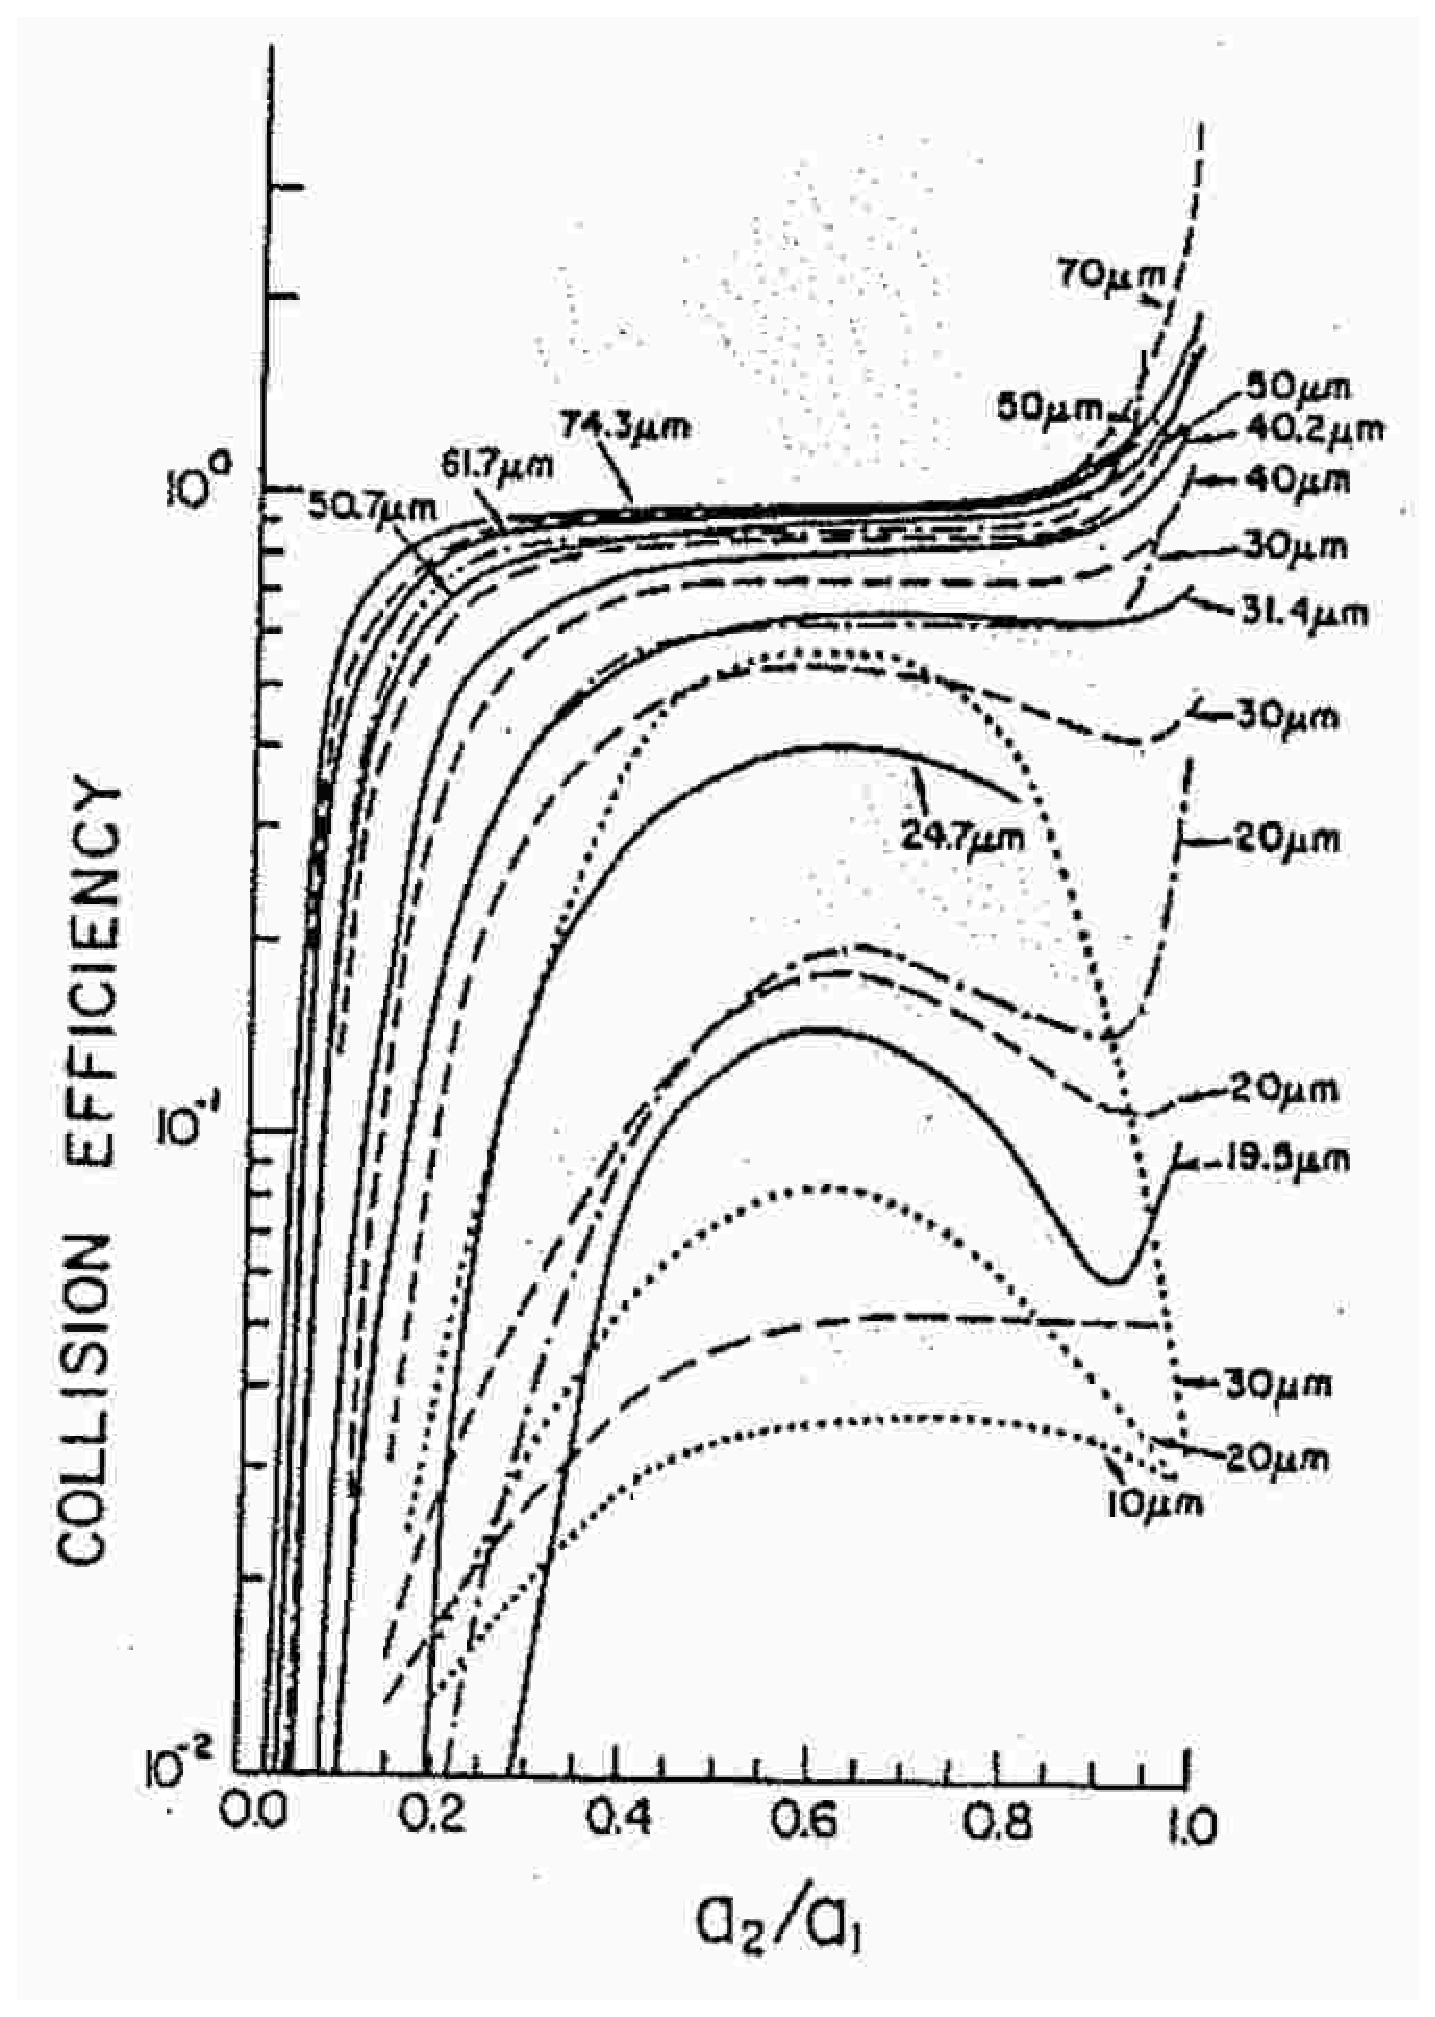
\includegraphics[width=0.5\linewidth,keepaspectratio]{CollisionEfficiency.eps}
            \caption{衝突係数の理論計算値。各曲線の値は大きい側の粒子半径を示す。}\label{CollisionEfficiency}
            \end{figure}
              この図では、捕捉される粒子が小さい場合の衝突係数が小さくなることがわかるが、このようになる理由を述べなさい。
        \item 下線部(c)について、観測される降水現象が雪になるか雨になるかは、図のように観測場所の湿度と気温に依存する。
            \begin{figure}[ptbh]
            \centering
            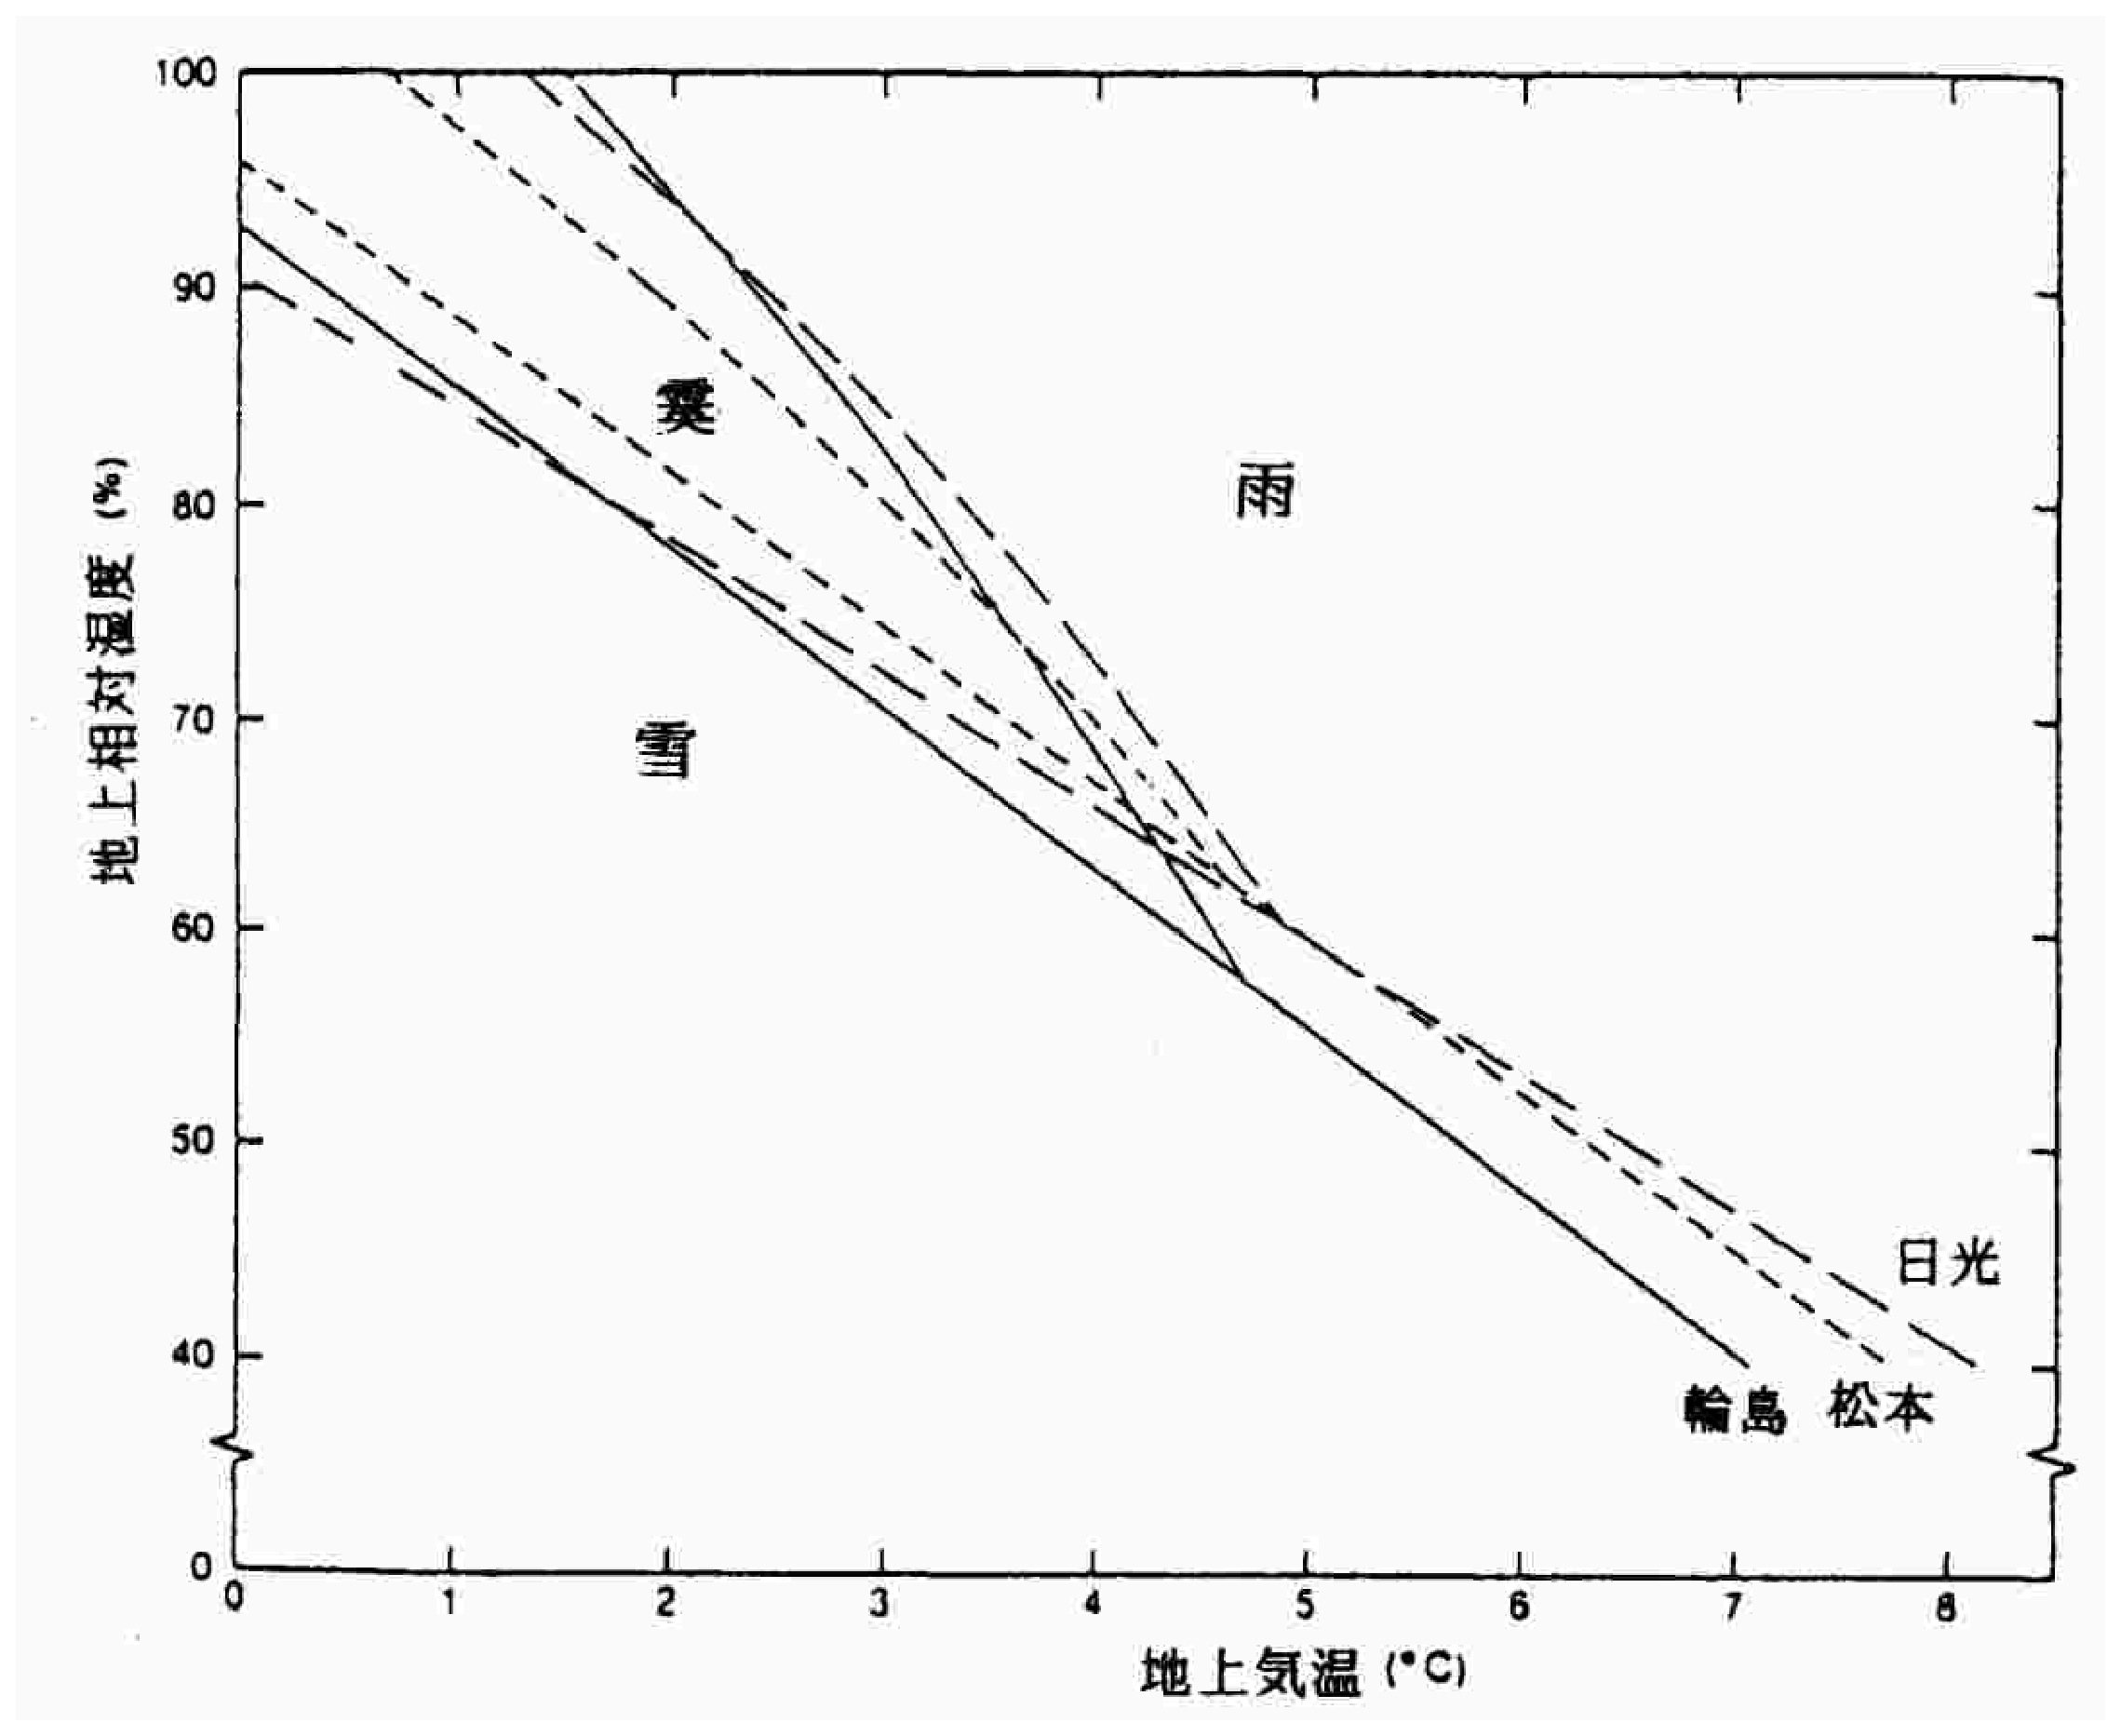
\includegraphics[width=0.5\linewidth,keepaspectratio]{RainSnow.eps}
            \caption{温度・湿度による雨と雪の種別。気象学会誌「天気」の「天気の教室 雪と雨をわけるもの」(松尾敬世)より引用}\label{RainSnow}
            \end{figure}
              図から明らかな通り、雪になるのは気温や湿度が低いほど有利であるが、その理由を述べなさい。\clearpage
        \end{enumerate}

    \item 教科書図4.2の曲線はケーラー曲線と呼ばれる。この下限はRaoultの法則により、上限はKelvinの法則により与えられる。
        この問題では、ケーラー曲線を実際にかいてみよう。
        \begin{enumerate}[(1)]
        \item 半径$r$の球形の水滴に対し、Raoultの法則が成り立つと仮定する。今、この水滴が吸湿性エーロゾルの希薄溶液であるとき、$e'/e$を$r$の関数として表しなさい。係数部分は定数$b$として良い。
        \item 前問で求めた$e$は球形水滴に対する飽和水蒸気圧であるから、Kelvinの式の$e_r$に相当している。このことを踏まえ、Kelvinの式の半径無限大の水滴に対する$e$を$e_\infty$と記す時、$e'/e_\infty$を$r$の関数として表しなさい。
        \item 前問の指数関数内の$r$に対する係数を$a$と表すことにする。指数関数を線形近似し、$ab$の項をneglectすることにより、$e'/e_\infty$を$r,a,b$及び定数のみによる式に書き直しなさい。
        \item 以上の議論を踏まえ、99\%から過飽和度1\%程度の範囲のケーラー曲線を描きなさい。\\
        \end{enumerate}

    \item 古来、天気は神が定めるものとして、渇水時などには雨乞いの儀式が行われた。日本各地で広く行われた形態としては、山野、特に山頂で火を焚き、鉦や太鼓を鳴らして大騒ぎする形態が多いとされている。
        \begin{enumerate}[(1)]
        \item この形態の雨乞いについて、火を焚くことは科学的にも有効と考えられるが、それは何故か説明しなさい。
        \item 同様の形態の雨乞いが有用でないと思われるのはどのような気候の地域か、根拠とともに述べなさい。
        \end{enumerate}

\end{problems}

\section{答案}
\begin{problems}
% 以下に解答を作成してGit Push。
\item 

\item 

\item 

\end{problems}

\section{読書案内}
大気熱力学及び降水の物理に関する邦書はあまり多くない。洋書であるが、Rogers,Yauは古典的な名著とされている。
\begin{itemize}
\item 水野量 2000 "雲と雨の気象学" 朝倉書店
\item 村上正隆 2021 "日本の降雪" 朝倉書店
\item 武田喬男,安田延寿,上田豊,藤吉康志 1992 "水の気象学" 東大出版
\item R.R.Rogers,M.K.Yau 1989 "A Short Course in Cloud Physics" Butterworth-Heinemann
\end{itemize}

\end{document}

